\subsection{Open Collaboration in the Classroom}
\label{opencollaborationintheclassroom}

From preliminary work including personal engagement in an open collaboration project and individual assignments, one main goal of the class is to produce a relevant collective report with no {\it ex-ante} guidelines and with self-organization as the default more. Instructors act as ``benevolent dictators" only when required or if extensive discussion are likely the impede to finish the report on time. We report on the main (self-)organization steps for this report.

\begin{enumerate}
  \item Collective report topic brainstorming {\bf (self-organized)} : recall the date and what has triggered a change in the syllabus
  \item Decision to design a survey {\bf (instructors)} : by the instructors
  \item Survey design {\bf (self-organized)} : question design (one by student) + categories
  \item Survey answering {\bf (instructors)} : everyone had to take the survey within a precise time window (recall it)
  \item Survey analysis {\bf (instructors)} :  each of us was asked to perform an analysis of her own proposed question(s).
  \item Report Latex format {\bf (instructors)} : choice for Latex by the instructors
  \item Learning Latex {\bf (self-organized)} : no crash course for Latex was provided in class. Those most confident with compiling installed or used Latex on their own computer. Others just edited the text without compiling. Mistakes would be corrected by those who could compiled the Latex code. The compiled document was sent regularly as a pdf to the mailing list. Surprisingly, there were little mistakes that prevented from compilation. On the other hand, the report has little sophisticated figures and tables.
  \item Producing a first chunk {\bf (instructors)} : all students were required to produce and commit a short paragraph commenting on the results provided to their own survey question.  
  \item Group formation to handle parts of the report {\bf (self-organized)} : 
  \item Production by groups {\bf (self-organized)} : To handle more integrative concepts and coherence of larger sections, groups were formed on a {\it task selection} basis during a class lab. Groups then drafted their sections on various collaborative editing platforms (e.g. etherpad, Google Docs). Sections built on chunks were finally uploaded as Latex files on the class repository.
  \item Peer-review {\bf (self-organized)} : Each section was reviewed by one or multiple peers until the document converged 
  \item Editing harmonization {\bf (self-organized)} : To harmonize editing -- to the extent it was possible -- we have tried to implement a few rules (use ``we", present tense by default).
\end{enumerate}


%\begin{figure}[ht!]
%\centering
%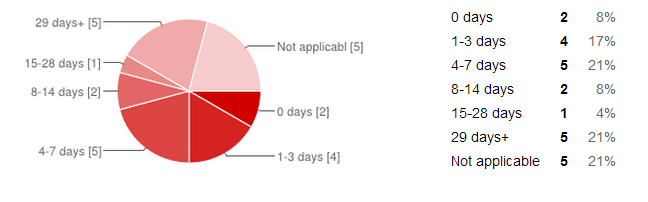
\includegraphics[width=90mm]{chapters/img/lurking_response.png}
%\caption{Network of survey topic organization and Progressive merging}
%\label{overflow}
%\end{figure}


\mysubsubsection{Other Patterns of Self-Organization}\\ 
We have found other patterns of self-organization in the class. To handle the large flows of commits for assignments, and commits to the report, committer rights were granted to volunteers, who reviewed and merged changes. Besides 
the official class website and github repository \cite{classweb2013}, we have used a variety of ad-hoc tools to help coordinate production and interactions. Etherpad, Google Docs, Google Forms are among these tools. A third pattern of self-organization is the way the instructors have tried to be less interventionist, precisely to allow (resp. force) more self-organization from the class. The effects of this policy are discussed later on in Section \ref{}.


